Os motores de passo híbrido, ou \textit{Hybrid Stepper Motor} (da sigla \textbf{HSM}) como são citados na literatura, são comumente utilizados em aplicações que demandam de alta precisão com motores de alimentação em corrente contínua \cite{ieeeRusso}.
	
	O HSM, como será referido neste trabalho, combina as vantagens do motor de relutância variável (\textit{Variable Reluctance Motor}, da sigla \textbf{VRM}) e do motor de imã permanente (\textit{Permanent Magnet Motor}, da sigla \textbf{PMM}).
	
	Um exemplo de um motor de passo híbrido simples é apresentado na Fig. \ref{HSMgrafico}.
	
	\begin{figure}[H]
		\centering
		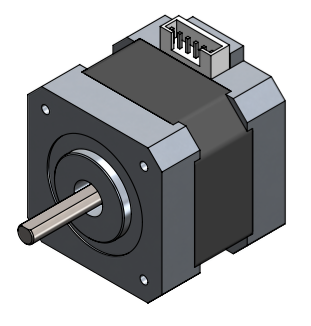
\includegraphics[scale=0.3]{Images/HSMmodel.png}
		\caption{Motor de passo híbrido 17HS3001-20B (RP One Labs)}
		\label{HSMgrafico}
	\end{figure}  
	
	Como em outros motores elétricos, o motor de passo híbrido é composto por um estator e um rotor. Entretanto, as características do HSM compõem as funcionalidades principais dos dois motores, VRM e PMM, que o tornam bastante preciso e eficiente. Devido a esta particularidade, o motor em questão é denominado de \textbf{híbrido}.
	
	As características construtivas, princípio de funcionamento, modelagem matemática e acionamento do motor serão apresentadas posteriormente, no decorrer deste trabalho. 